\begin{frame}{Talk Outline}
  \research{\citet{Wiseman2016a}}

  \begin{enumerate}
  \item Background: Core Model and Implementation
    \air
  \item \textbf{Work 1}: Rethinking Model Training (\textit{Beam Search Optimization})
    \air

  \item Work 2: Rethinking  Generation  (\textit{Learning Neural Templates})
    \air

  \item Future Directions
  \end{enumerate}
\end{frame}


% \begin{frame}{Part 3: Structured Modeling}
%   \begin{center}
%     \scalebox{2}{
%   \begin{tikzpicture}

%     \node<1> at (10mm, 15mm){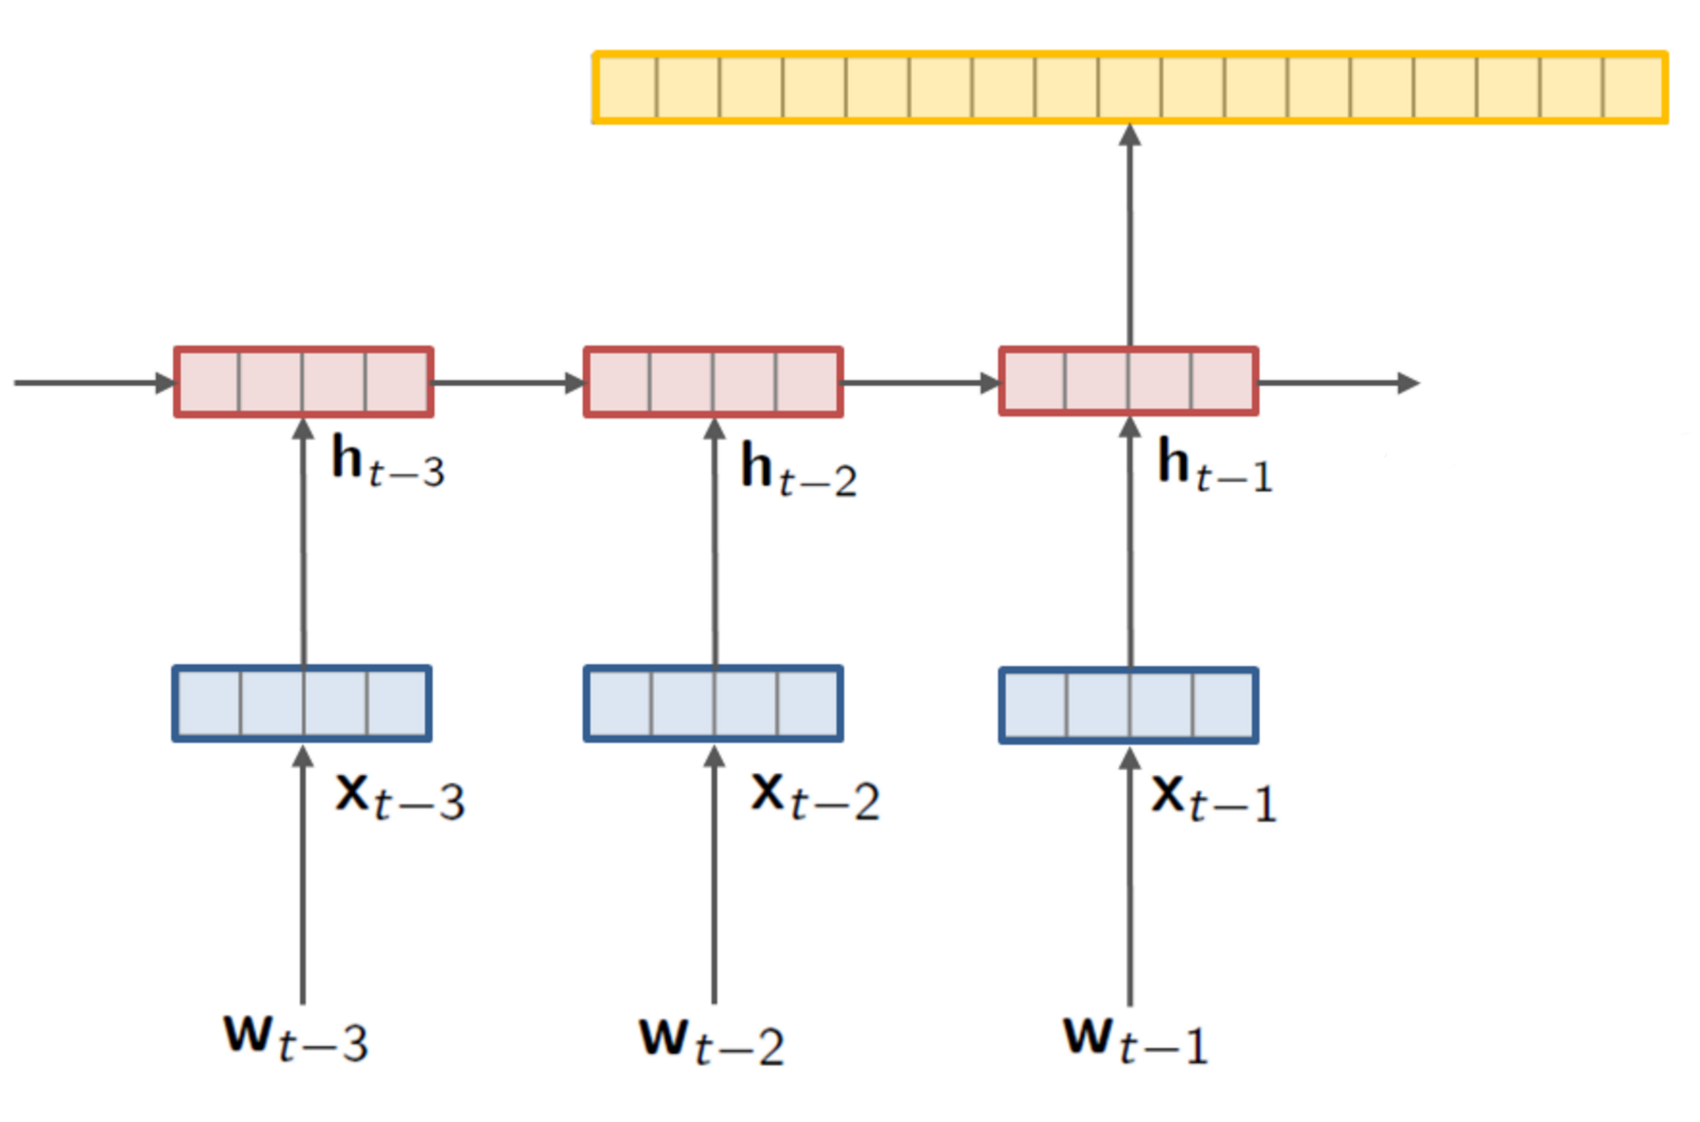
\includegraphics[width=3cm]{rnnlm6}};
%     \node[draw,  thick, rounded corners, scale=0.5] (ana) at (-15mm, 15mm) {Analysis};
%     \node[draw,  fill=yellow, thick, rounded corners,scale=0.5] (meth) at (0mm, 30mm) {\ Methods\phantom{p}};
%     \node[draw,  thick, rounded corners,scale=0.5] (app) at (25mm, 30mm) {Applications};
%     \node[draw, thick, rounded corners, scale=0.5] (und) at (35mm, 15mm) {Understanding};
%     \node[draw, fill=yellow, thick, rounded corners, scale=0.5] (dep) at (25mm, 0mm){Deployment};

%     \node[draw, thick, rounded corners,scale=0.5] (imp) at (0, 0) {Implementation};

%     \draw (ana) -- (meth) --(app) -- (und) -- (dep) -- (imp) -- (ana);

%   \end{tikzpicture}
% }
%   \end{center}
% \end{frame}


\begin{frame}{Beam Search Optimization}
  Research Goal: Can we learn parameters $\theta$ to target text generation problems?

    \[ {y^*_{1:T}} = \argmax_{y_{\tikzmark{opt}1:T}} {f}(y_{1:T}, \tikzmark{input}{x}; \tikzmark{nn}{\alert{\theta}}) \]


  \begin{itemize}

  \item Input {$x$},  \textit{what to talk about}
    \air

  \item Output text {$y^*_{1:T}$}, \textit{how to say it}
    \air

  \item Scoring model {$f(.; \theta)$}, learned from data
  \end{itemize}

\end{frame}


\begin{frame}{Training Encoder-Decoder}
  Parameters $\theta$ are trained to predict the next word \textit{given the true history.}

  \begin{center}
  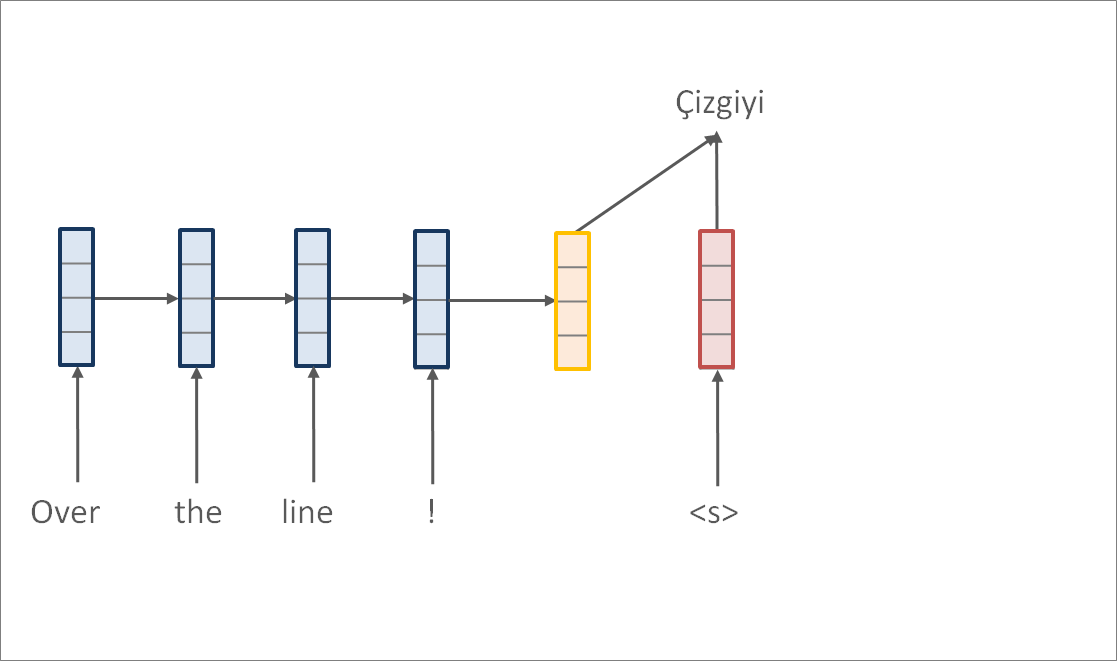
\includegraphics[height=3.5cm, trim={12cm 3cm 7cm 0.5cm}, clip]{nmt-noattn-4}
  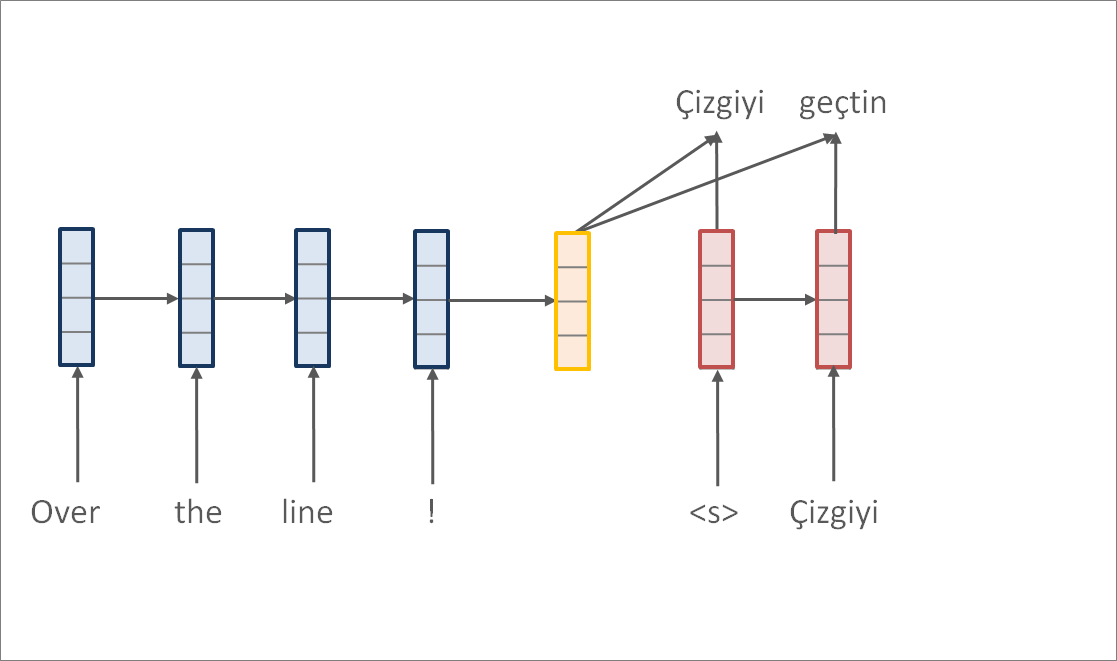
\includegraphics[height=3.5cm, trim={12cm 3cm 3cm 0.5cm}, clip]{nmt-noattn-6}
  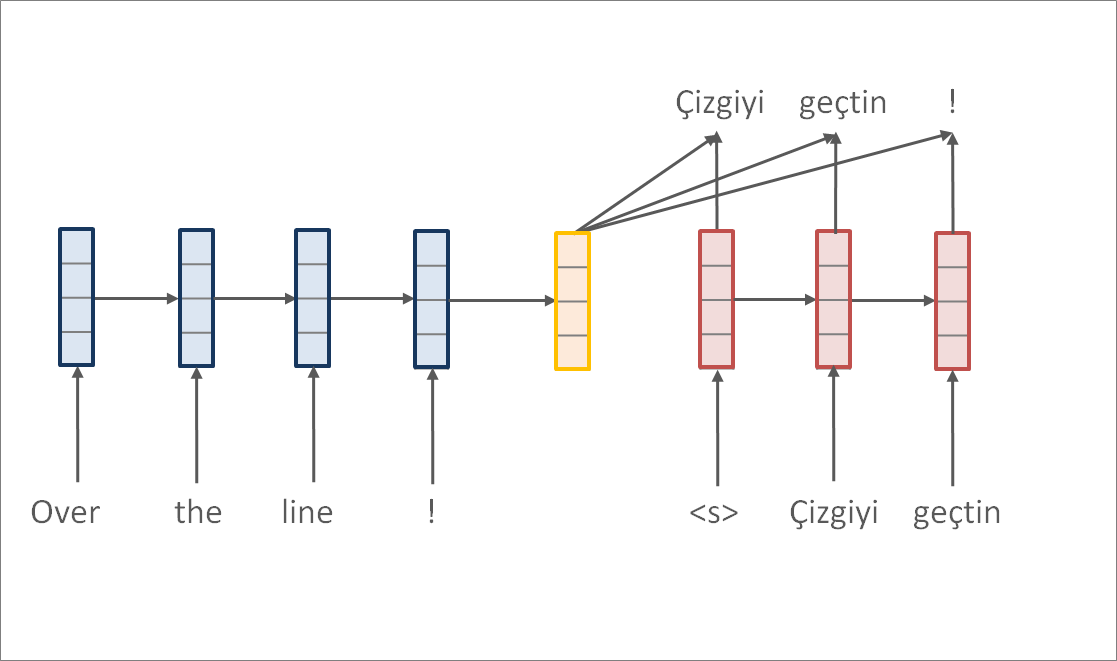
\includegraphics[height=3.5cm, trim={12cm 3cm 0.5cm 0.5cm}, clip]{nmt-noattn-7}
  % 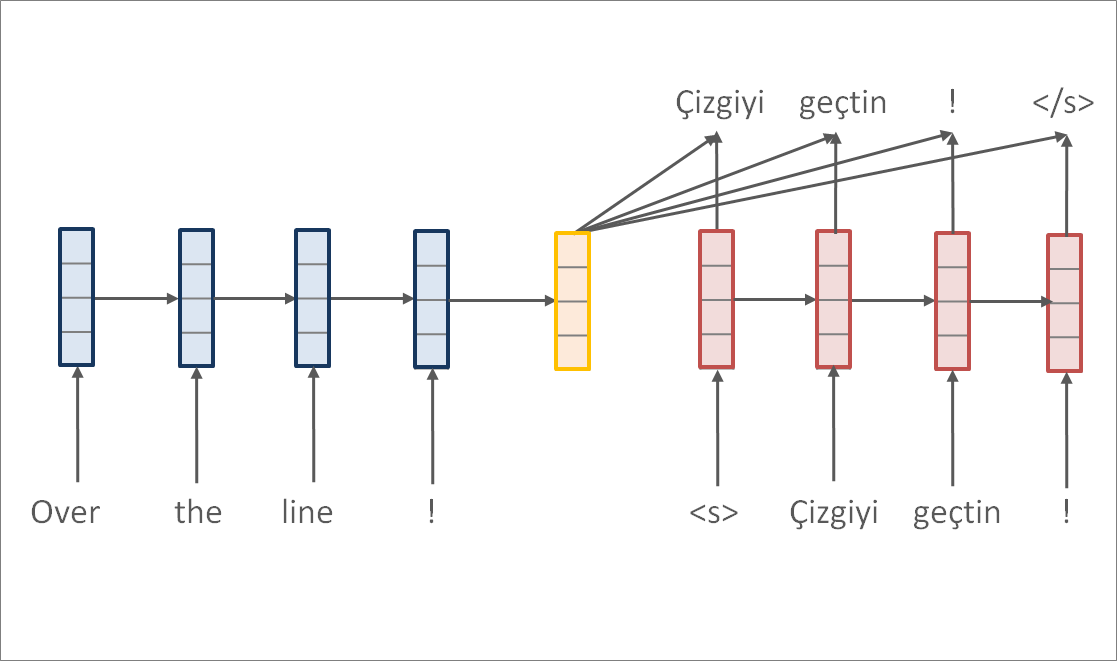
\includegraphics[height=3.5cm, trim={12cm 3cm 0.5cm 0.5cm}, clip]{nmt-noattn-8}
  \end{center}
  \pause

  Objective is identical to \textcolor{redpurple}{multiclass classification}.
  \[ {\cal L}(\theta) = -\sum_{t} \log p(y_t |  y_{1:t-1}, x; \theta) \]
\end{frame}

\begin{frame}{Generating with Encoder-Decoder}
  Parameters $\theta$ are deployed to predict the next word \textit{given a hypothesized history}.


  \begin{center}
  % 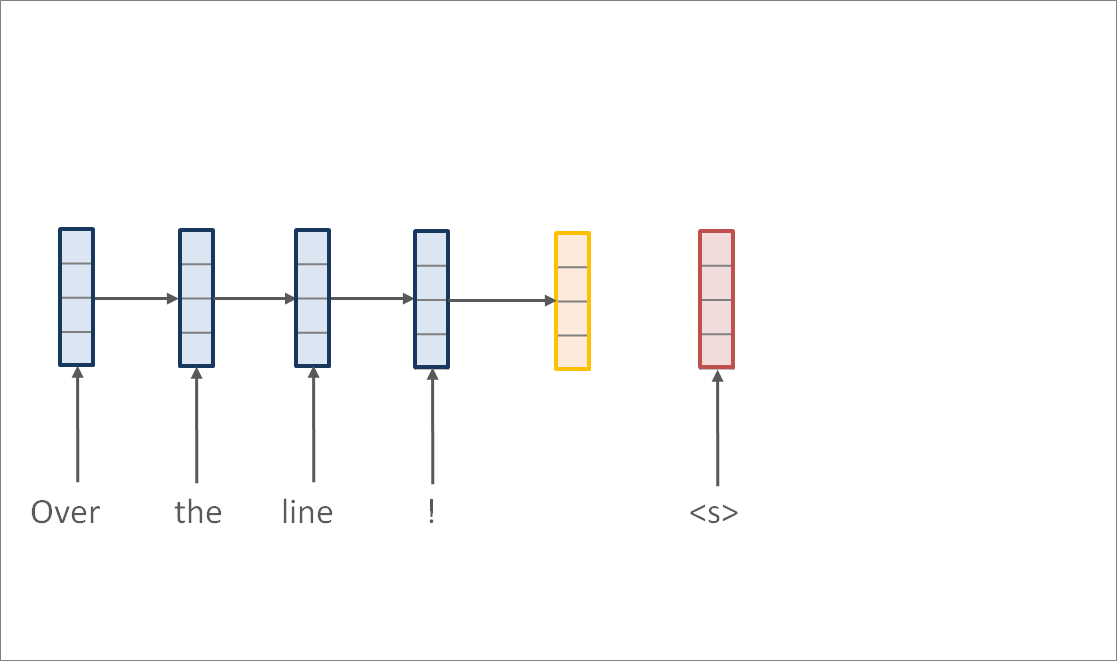
\includegraphics[height=3.5cm, trim={12cm 3cm 7cm 0.5cm}, clip]{nmt-noattn-3}
  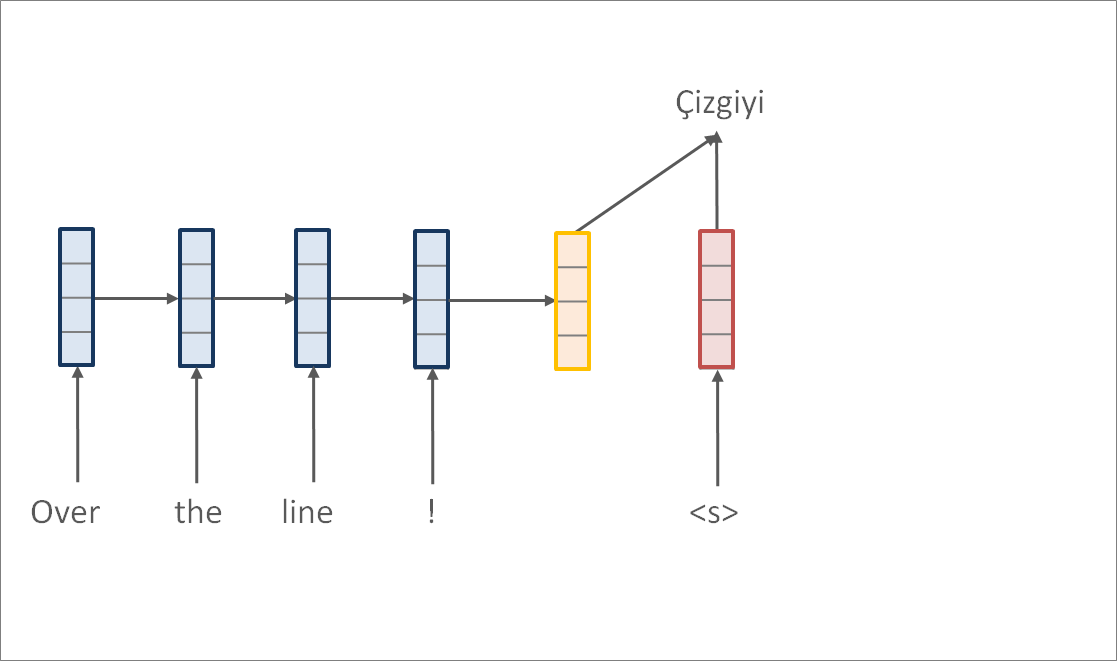
\includegraphics[height=3.5cm, trim={12cm 3cm 7cm 0.5cm}, clip]{nmt-noattn-4}
  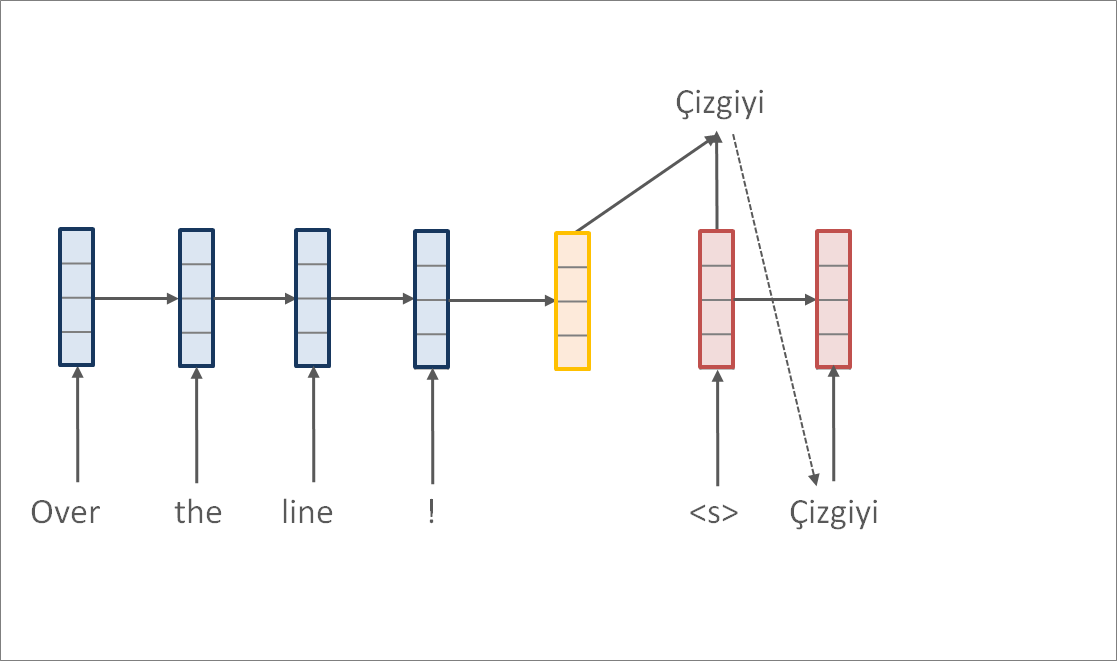
\includegraphics[height=3.5cm, trim={12cm 3cm 0.5cm 0.5cm}, clip]{nmt-noattn-5}
  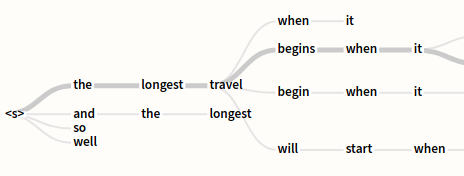
\includegraphics[width=7cm]{beam}
  \end{center}

  Requires  predicting best sequence
  \[ y^*_{1:T} = \argmax_{y_{1:T}} f(y_{1:T}; \theta) = \argmax_{y_{1:T}} \sum_{t} \log p(y_{t} | y_{1:t-1}, x; \theta) \]
  % \pause

  Intractable to solve exactly $O(\text{\#vocab} ^T)$

\end{frame}

\begin{frame}[fragile]{Standard Heuristic Method:  Beam Search}
    \begin{center}
  \begin{tikzpicture}[transform canvas = {scale=0.8}]
    \tikzstyle{beam}=[draw, minimum height=0.6cm, anchor=base, text height=5, text depth=0, minimum width=1.5cm,thin, rounded corners, line width=0.03cm]
   \tikzstyle{mat}=[draw=white]
    \tikzset{>=stealth',every on chain/.append style={join},
      every join/.style={->}}


       \begin{scope}
   \matrix (G) [matrix of nodes, nodes={beam},inner sep=1mm,row sep=0.03cm, column sep=0.8cm ] {
    \node<1->(G-1-1){a}; & \node<2->(G-1-2){red}; & \node<3->(G-1-3){dog}; & \node<4->(G-1-4){smells}; & \node<5->(G-1-5){home};  & \node<6->(G-1-6){today}; \\
    \node<1->(G-2-1){the}; & \node<2->(G-2-2){dog}; & \node<3->(G-2-3){dog}; & \node<4->(G-2-4){barks}; & \node<5->(G-2-5){quickly}; & \node<6->(G-2-6){Friday}; \\
    \node<1->(G-3-1){red}; & \node<2->(G-3-2){blue}; & \node<3->(G-3-3){cat}; &  \node<4->(G-3-4){walks}; & \node<5->(G-3-5){straight}; & \node<6->(G-3-6){now}; \\    };

    \only<2->{
      \draw[->] (G-1-1.east) -> (G-1-2.west);
      \draw[->] (G-2-1.east) -> (G-2-2.west);
      \draw[->] (G-1-1.east) -> (G-3-2.west);
      \draw[double, line width=0.03cm] (G-3-1.south west) -- (G-3-2.south east);
    }

    \only<3->{
      \draw[->] (G-1-2.east) -> (G-2-3.west);
      \draw[->] (G-3-2.east) -> (G-3-3.west);
      \draw[->] (G-3-2.east) -> (G-1-3.west);
      \draw[double, line width=0.03cm] (G-3-1.south west) -- (G-3-3.south east);
    }

 \only<4->{
    \draw[->] (G-1-3.east) -> (G-3-4.west);
    \draw[->] (G-2-3.east) -> (G-2-4.west);
    \draw[->] (G-1-3.east) -> (G-1-4.west);
    \draw[double, line width=0.03cm] (G-3-1.south west) -- (G-3-4.south east);
}
 \only<6->{
    \draw[->] (G-1-5.east) -> (G-1-6.west);
    \draw[->] (G-1-5.east) -> (G-3-6.west);
    \draw[->] (G-2-5.east) -> (G-2-6.west);
    \draw[double, line width=0.03cm] (G-3-1.south west) -- (G-3-6.south east);
}

 \only<5->{
    \draw[->] (G-3-4.east) -> (G-1-5.west);
    \draw[->] (G-3-4.east) -> (G-2-5.west);
    \draw[->] (G-3-4.east) -> (G-3-5.west);
    \draw[double, line width=0.03cm] (G-3-1.south west) -- (G-3-5.south east);
}
         \node[left=0.2cm of G]{K = 3};
         \node[below=0.1cm of G]{T};

\end{scope}
\end{tikzpicture}
    \end{center}

\air
    \air

\air

\visible<7->{
   \begin{enumerate}
   \item Compute the score of every possible next word.
     \[f(y_t, y_{1:t-1}^{(k)}) \gets \log p(y_{t}\ |\ y^{(k)}_{1:t-1}, x) + \log p(y^{(k)}_{1:t-1} \ |\  x) \]
     \pause
   \item Prune to only the $K$ highest-scoring,
     \[y_{1:t}^{(1:K)} \gets K\argmax_{y_{1:t}} f(y_t, y_{1:t-1}^{(k)})\]
   \end{enumerate}
}

  % \begin{enumerate}
  % \item Start with $K$ partial starting hypotheses $\wvec^{(1:K)}$
  % \item For timesteps $t$ from  $1$ to $T$:
  %  \begin{enumerate}
  %  \item Compute for all $k, \wvec_{t}$
  %    \[s(\wvec_t, k) \gets \log p(\wvec_{t} | \wvec^{(k)}_{1:t-1}, \cvec; \theta) + \log p(\wvec^{(k)}_{1:t-1}| \cvec;\theta) \]
  %  \item Save $K$ highest scoring target sequences
  %    \[\wvec_{1:t+1}^{(1:K)} \gets K\arg\max_{\wvec_t, k} s(\wvec_t, k)\]
  %  \end{enumerate}
  % \end{enumerate}
  \pause
  % \begin{itemize}
  % \item Note: Requires computing $p(\wvec_{t} | \wvec^{(k)}_{1:t-1}, \cvec; \theta)$ for many  $\wvec^{(k)}_{1:t-1}$
  % \end{itemize}
\end{frame}

% \begin{frame}[fragile]{Beam Search Example} ($K=3$)


%     \begin{center}
%   \begin{tikzpicture}[transform canvas = {scale=0.8}]
%     \tikzstyle{beam}=[draw, minimum height=0.6cm, anchor=base, text height=5, text depth=0, minimum width=1.5cm,thin, rounded corners, line width=0.03cm]
%    \tikzstyle{mat}=[draw=white]
%     \tikzset{>=stealth',every on chain/.append style={join},
%       every join/.style={->}}


%        \begin{scope}

%    \matrix (G) [matrix of nodes, nodes={beam},inner sep=1mm,row sep=0.03cm, column sep=0.8cm ] {
%     \node<1->(G-1-1){a}; & \node<2->(G-1-2){red}; & \node<3->(G-1-3){dog}; & \node<4->(G-1-4){smells}; & \node<5->(G-1-5){home};  & \node<6->(G-1-6){today}; \\
%     \node<1->(G-2-1){the}; & \node<2->(G-2-2){dog}; & \node<3->(G-2-3){dog}; & \node<4->(G-2-4){barks}; & \node<5->(G-2-5){quickly}; & \node<6->(G-2-6){Friday}; \\
%     \node<1->(G-3-1){red}; & \node<2->(G-3-2){blue}; & \node<3->(G-3-3){cat}; &  \node<4->(G-3-4){runs}; & \node<5->(G-3-5){straight}; & \node<6->(G-3-6){now}; \\    };

%     \only<2->{
%       \draw[->] (G-1-1.east) -> (G-1-2.west);
%       \draw[->] (G-2-1.east) -> (G-2-2.west);
%       \draw[->] (G-1-1.east) -> (G-3-2.west);
%       \draw[double, line width=0.03cm] (G-3-1.south west) -- (G-3-2.south east);
%     }

%     \only<3->{
%       \draw[->] (G-1-2.east) -> (G-2-3.west);
%       \draw[->] (G-3-2.east) -> (G-3-3.west);
%       \draw[->] (G-3-2.east) -> (G-1-3.west);
%       \draw[double, line width=0.03cm] (G-3-1.south west) -- (G-3-3.south east);
%     }

%  \only<4->{
%     \draw[->] (G-1-3.east) -> (G-3-4.west);
%     \draw[->] (G-2-3.east) -> (G-2-4.west);
%     \draw[->] (G-1-3.east) -> (G-1-4.west);
%     \draw[double, line width=0.03cm] (G-3-1.south west) -- (G-3-4.south east);
% }
%  \only<6->{
%     \draw[->] (G-1-5.east) -> (G-1-6.west);
%     \draw[->] (G-1-5.east) -> (G-3-6.west);
%     \draw[->] (G-2-5.east) -> (G-2-6.west);
%     \draw[double, line width=0.03cm] (G-3-1.south west) -- (G-3-6.south east);
% }

%  \only<5->{
%     \draw[->] (G-3-4.east) -> (G-1-5.west);
%     \draw[->] (G-3-4.east) -> (G-2-5.west);
%     \draw[->] (G-3-4.east) -> (G-3-5.west);
%     \draw[double, line width=0.03cm] (G-3-1.south west) -- (G-3-5.south east);
% }

% \end{scope}
% \end{tikzpicture}
%     \end{center}
%     \air

% For timesteps $t$ from  $1$ to $T$:
%    \begin{enumerate}
%    \item Compute for all $k, \wvec_{t}$
%      \[f(\wvec_t, \wvec_{1:t-1}^{(k)}) \gets \log p(\wvec_{t} | \wvec^{(k)}_{1:t-1}, \cvec) + \log p(\wvec^{(k)}_{1:t-1}| \cvec) \]
%    \item Replace the $K$ highest scoring target sequences
%      \[\wvec_{1:t}^{(1:K)} \gets K\argmax_{\wvec_{1:t}} (\wvec_t, \wvec_{1:t-1}^{(k)})\]
%    \end{enumerate}

% \end{frame}


\begin{frame}{Theoretical Issues with Multiclass Training for Generation}
  \begin{enumerate}

  \item Exposure Bias
    \begin{itemize}
    \item Training conditions on true history, but generation uses predicted history.
    \end{itemize}
    \air
    \pause

  \item Label Bias  %\cite{Lafferty2001}
    \begin{itemize}
    \item Training is locally multiclass, but score is over entire sequences.
    \end{itemize}
    \air
    \pause


  \item Metric Bias
    \begin{itemize}
    \item Training uses multiclass classification, but evaluation uses n-gram match.
    \end{itemize}
    \air

  \end{enumerate}
\end{frame}

\begin{frame}{Beam Search Optimization}

  \textbf{Strategy:} Modify training to target each issue.

  \begin{itemize}
  \item Exposure Bias, Label Bias, Metric Bias

  \end{itemize}
\air
\air

  \textbf{Applications:}

  \begin{enumerate}
  \item Improvements in training with less supervision.
    \air
  \item  Effective methods for downscaling translation models.
    \air
  \end{enumerate}
\end{frame}


% \begin{frame}{\structure{Related Work:} Modify training data}
%   \air
%   \begin{itemize}
%   \item Data as Demonstrator \Cite{Venkatraman}, Scheduled Sampling \Cite{Bengio2015}
%   \end{itemize}
%   \air

%   \centerline{\structure{Related Work:} Use Reinforcement Learning}
%   \air
%   \begin{itemize}
%   \item MIXER \Cite{Ranzato2016}
%   \item Actor-Critic \Cite{Bahdanau2016}
%   \end{itemize}

%   \pause

%   Opinion:
%   \begin{itemize}
%   \item
%     DAD methods only address exposure bias,
%   \item RL is too strong a hammer .
%   \end{itemize}

%   % \begin{itemize}
%   % \item
%   % \end{itemize}
% \end{frame}

% \begin{frame}{Sequence-to-Sequence Learning as Beam Search Optimization}


%   Proposal: Directly modify the RNN training procedure to fix test biases.


%   % \begin{itemize}
%   % \item
%   % \end{itemize}
% \end{frame}

\begin{frame}{Modification 1: Beam Search at Training}

  \textbf{Goal:}  Fix Exposure Bias
    \begin{itemize}
    \item Train taking prediction into account.
    \end{itemize}
    \air
    \pause

   \textbf{Proposed Fix:}

   \begin{itemize}
   \item Run our beam search procedure during training (structured prediction)
     \air

   \item Update parameters only when true sequence becomes impossible to recover.
   \end{itemize}
   % \begin{enumerate}
   % \item Compute the score of every possible next word.

   %   \[f(y_t, y_{1:t-1}^{(k)}) \gets \log p(y_{t}\ |\ y^{(k)}_{1:t-1}, x) + \log p(y^{(k)}_{1:t-1} \ |\  x) \]

   % % \only<2>{
   % %   \[f(y_t, y_{1:t-1}^{(k)})  \gets  \structure{f(y_t, y_{1:t-1}^{(k)}, x; \theta)} \]}

   % \item Prune to only the $K$ highest-scoring,
   %   \[y_{1:t}^{(1:K)} \gets K\argmax_{y_{1:t}} f(y_t, y_{1:t-1}^{(k)})\]
   % \end{enumerate}
  % \begin{enumerate}
  % % \item Start with $K$ partial starting hypotheses $\wvec^{(1:K)}$
  % % \item For timesteps $t$ from  $1$ to $T$:
  %  \begin{enumerate}
  %  \item Compute for all $k, \wvec_{t}$
  %    \only<1>{
  %    \[f(\wvec_t, \wvec_{1:t-1}^{(k)}) \gets \alert{\log p(\wvec_{t} | \wvec^{(k)}_{1:t-1}, \cvec; \theta) + \log p(\wvec^{(k)}_{1:t-1}| \cvec;\theta)} \]
  %  }
  %  \only<2>{
  %    \[f(\wvec_t, \wvec_{1:t-1}^{(k)})  \gets  \structure{f(\wvec_t, \wvec_{1:t-1}^{(k)}, \cvec; \theta)} \]
  %  }
  %  \item Replace the  $K$ highest scoring target sequences
  %    \[\wvec_{1:t}^{(1:K)} \gets K\argmax_{\wvec_{1:t}} s(\wvec_t, \wvec_{1:t-1}^{(k)})\]
  %  \end{enumerate}
  % \end{enumerate}
\end{frame}

\begin{frame}{Modification 2: Global Scoring Function  }
  \textbf{Goal:}  Fix Label Bias
    \begin{itemize}
    \item Use a direct global scoring function.
    \end{itemize}
    \pause

  % \begin{center}
  %   % \structure{(Idea 1)} Replace local softmax with sequence scorer
  %   % \air
  %
  % \end{center}

    \air

  \textbf{Proposed Fix:}

  \begin{itemize}
  \item Replace $ \log p(y_{t} | y_{1:t-1}, x; \theta)$ with
    a directly learned function $f(y_{1:t}, x; \theta)$
  \end{itemize}
  \air

  \begin{center}
    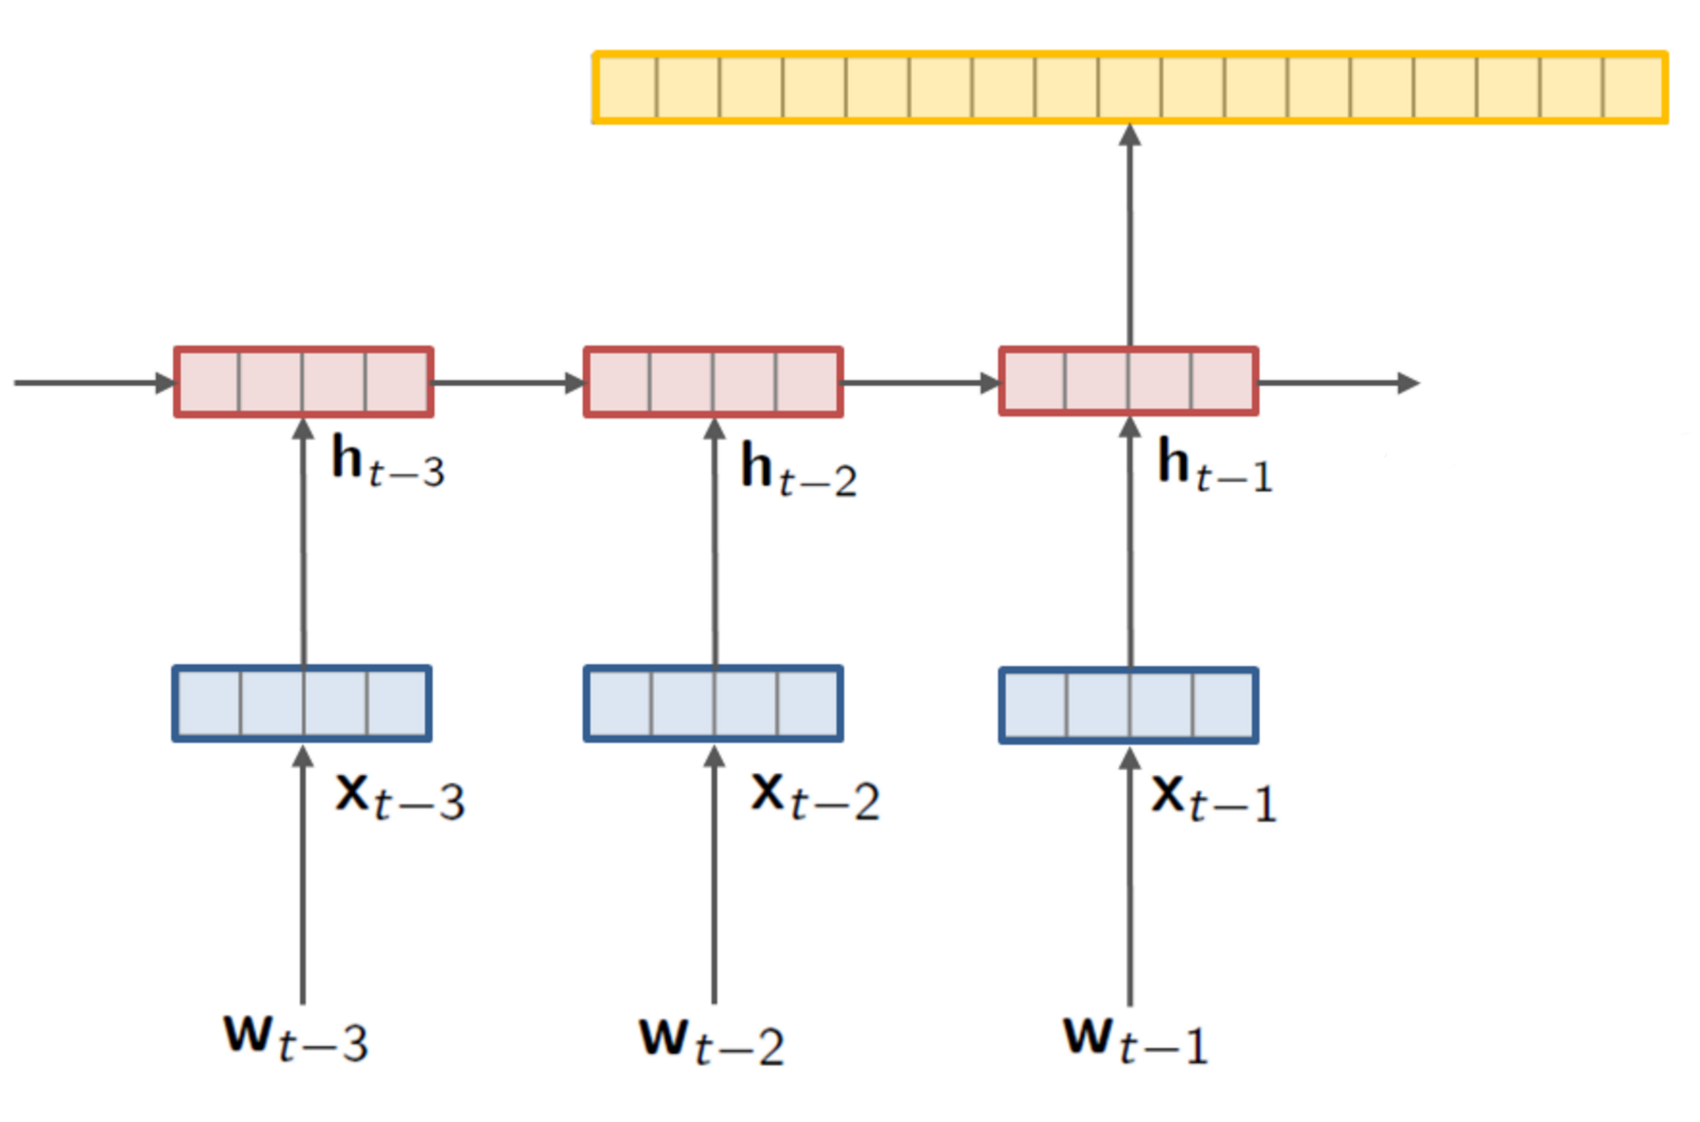
\includegraphics[width=0.5\textwidth, trim={0cm 18cm 0cm 0cm}, clip]{rnnlm6}
  \end{center}
\end{frame}



\begin{frame}{Modification 3: Train with Margin}

  \textbf{Goal:} Fix Metric Bias
    \begin{itemize}
    \item Incorporate a problem specific cost, e.g. ngrams
    \end{itemize}
\air
\pause

    \textbf{Proposed Fix:} Use a structured SVM-style training loss:
    \begin{itemize}
    \item Margin between ground truth sequence $\hat{y}$ and worst predicted sequence $y^{(K)}$
    \end{itemize}
    \begin{align*}
      \mathcal{L}&(\theta) = \sum_{t} \Delta(\hat{y}_{1:t}, y_{1:t}^{(K)}) \left[1 - f(\hat{y}_t, \hat{y}_{1:t-1}, x) +  f(y_t^{(K)}, y_{1:t-1}^{(K)}, x) \right]
    \end{align*}

    \begin{itemize}
    \item Slack-rescaled, margin-based sequence criterion, at each time step.
    \item $\Delta$ is a task specific sequence cost, i.e. ngram-mismatch
    \end{itemize}

  \end{frame}

\begin{frame}{Extension: Train with Constraints}
  (Constraints)

\end{frame}




\begin{frame}[fragile]{Beam Search Optimization: Training Example}
  \begin{center}
    \begin{center}

    \end{center}
    \air
    \air
    \air
    \air

\

  \begin{tikzpicture}[transform canvas = {scale=0.8}]
  \tikzstyle{beam}=[draw, minimum height=0.6cm, anchor=base, text height=5, text depth=0, minimum width=1.5cm,thin, rounded corners, line width=0.03cm]
  \tikzstyle{mat}=[draw=white]
\tikzset{>=stealth',every on chain/.append style={join},
         every join/.style={->}}


       % \node[draw = white, yshift=1.8cm]{Time Step};
       %\node[draw = white, xshift=-7.5cm, yshift=0.5cm]{Beam:};
       \begin{scope}


   \matrix (G) [matrix of nodes, nodes={beam},inner sep=1mm,row sep=0.03cm, column sep=0.8cm ] {
    \node<1->[fill=yellow](G-1-1){\textcolor{black}{a}}; \node<4->[fill=yellow](G-1-1){\textcolor{black}{a}}; & \node<2->[fill=yellow](G-1-2){red}; \node<4->[fill=yellow](G-1-2){red}; & \node<3->[](G-1-3){\textcolor{black}{dog}}; \node<4->[fill=red!20](G-1-3){\textcolor{black}{dog}}; & \node<4->(G-1-4){smells}; & \node<5->[](G-1-5){{home}}; \node<6->[fill=red!20](G-1-5){{home}};  & \node<6->[](G-1-6){{today}}; \\
    \node<1->(G-2-1){the}; & \node<2->(G-2-2){dog}; & \node<3->[fill=yellow](G-2-3){dog}; & \node<4->(G-2-4){barks}; & \node<5->[fill=yellow](G-2-5){quickly}; & \node<6->(G-2-6){Friday}; \\
    \node<1->(G-3-1){red}; & \node<2->[](G-3-2){\textcolor{black}{blue}}; \node<4->[fill=red!20](G-3-2){\textcolor{black}{blue}}; & \node<3->(G-3-3){cat}; &  \node<4->[fill=red!20](G-3-4){\textcolor{black}{barks}}; & \node<5->(G-3-5){straight}; & \node<6->[fill=red!20](G-3-6){now}; \\
    & & & \node<4->[fill=yellow](G-4-4){runs}; & & \node<6->[fill=yellow](G-4-6){today}; \\
    };

    \only<2->{
      \draw[->] (G-1-1.east) -> (G-1-2.west);
      \draw[->] (G-2-1.east) -> (G-2-2.west);
      \draw[->] (G-1-1.east) -> (G-3-2.west);
      \draw[double, line width=0.03cm] (G-3-1.south west) -- (G-3-2.south east);
    }

    \only<3->{
      \draw[->] (G-1-2.east) -> (G-2-3.west);
      \draw[->] (G-3-2.east) -> (G-3-3.west);
      \draw[->] (G-3-2.east) -> (G-1-3.west);
      \draw[double, line width=0.03cm] (G-3-1.south west) -- (G-3-3.south east);
    }

 \only<4->{
    \draw[->] (G-2-3.east) -> (G-4-4.west);
    \draw[->] (G-1-3.east) -> (G-3-4.west);
    \draw[->] (G-2-3.east) -> (G-2-4.west);
    \draw[->] (G-1-3.east) -> (G-1-4.west);
    \draw[double, line width=0.03cm] (G-3-1.south west) -- (G-3-4.south east);
}
 \only<6->{
    \draw[->] (G-1-5.east) -> (G-1-6.west);
    \draw[->] (G-1-5.east) -> (G-3-6.west);
    \draw[->] (G-2-5.east) -> (G-2-6.west);
    \draw[->] (G-2-5.east) -> (G-4-6.west);
    \draw[double, line width=0.03cm] (G-3-1.south west) -- (G-3-6.south east);
}

    % \draw[->] (G-3-2.east) -> (G-3-3.west);
    % \draw[->] (G-3-2.east) -> (G-1-3.west);

 \only<5->{
    \draw[->, dashed] (G-4-4.east) -> (G-1-5.west);
    \draw[->, dashed] (G-4-4.east) -> (G-2-5.west);
    \draw[->, dashed] (G-4-4.east) -> (G-3-5.west);
    \draw[double, line width=0.03cm] (G-3-1.south west) -- (G-3-5.south east);
}

       \end{scope}
    % \draw(G-1-1.north east) rectangle (G-3-1.south west);
    % \draw(G-1-2.north east) rectangle (G-3-2.south west);

    % \begin{scope}[yshift=-2.8cm]

    %   \matrix (G) [matrix of nodes,nodes={beam}, inner sep=1mm,row sep=0.06cm,column sep=0.8cm ] {
    %     \node[fill=yellow](G-1-1){a}; & \node[fill=yellow](G-1-2){red}; & \node[fill=yellow](G-1-3){dog}; & \node[fill=yellow](G-1-4){runs}; & \node[fill=yellow](G-1-5){quickly}; & \node[fill=yellow](G-1-6){today}; \\
    %      & \node[fill=lightgray](G-2-2){\textcolor{blue}{blue}}; & \node[fill=lightgray](G-2-3){\textcolor{blue}{dog}}; & \node[fill=lightgray](G-2-4){\textcolor{blue}{barks}}; & \node[fill=lightgray](G-2-5){\textcolor{red}{home}}; & \node[fill=lightgray](G-2-6){\textcolor{red}{today}}; \\
    %   };
    % \draw[->] (G-1-1.east) -> (G-1-2.west);
    % \draw[->] (G-1-2.east) -> (G-1-3.west);
    % \draw[->] (G-1-3.east) -> (G-1-4.west);
    % \draw[->] (G-1-4.east) -> (G-1-5.west);
    % \draw[->] (G-1-5.east) -> (G-1-6.west);

    % \draw[->] (G-1-1.east) -> (G-2-2.west);
    % \draw[->] (G-2-2.east) -> (G-2-3.west);
    % \draw[->] (G-2-3.east) -> (G-2-4.west);
    % \draw[->] (G-1-4.east) -> (G-2-5.west);
    % \draw[->] (G-2-5.east) -> (G-2-6.west);

    % \end{scope}
\end{tikzpicture}
  \end{center}
  \air
  \air
  \air
% \begin{align*}
%  \mathcal{L}&(\theta) = \sum_{t} \Delta(\wvec_{1:t}, \wvec_{1:t}^{(K)}) \left[1 - f(\wvec_t, \wvec_{1:t-1}, \cvec) +  f(\wvec_t^{(K)}, \wvec_{1:t-1}^{(K)}, \cvec) \right]
% \end{align*}

  \begin{itemize}
  \item \textcolor{orange}{True}: ground-truth sequence $\hat{y}$
  \item<4> \textcolor{red}{Predicted}: lowest-scoring prefix  $y^{(K)}$
  \end{itemize}
  % Strategy: if true falls off beam, restart from ground truth (learning as search optimization \cite{daume05learning})
\end{frame}

\begin{frame}[fragile]{Parameter Updates: Structured Backpropagation}
  \begin{center}

  \air
  \air



  \begin{tikzpicture}[transform canvas = {scale=0.8}]
    \tikzstyle{beam}=[draw, minimum height=0.6cm, anchor=base, text height=5, text depth=0, minimum width=1.5cm,thin, rounded corners, line width=0.03cm]
    \tikzstyle{mat}=[draw=white]
    \tikzset{>=stealth',every on chain/.append style={join},
      every join/.style={->}}


       % \node[draw = white, yshift=1.8cm]{Time Step};
       %\node[draw = white, xshift=-7.5cm, yshift=0.5cm]{Beam:};
       \begin{scope}


   \matrix (G) [matrix of nodes, nodes={beam},inner sep=1mm,row sep=0.03cm, column sep=0.8cm ] {
     \node[fill=yellow](G-1-1){\textcolor{blue}{a}}; & \node[fill=yellow](G-1-2){red}; & \node[fill=lightgray](G-1-3){\textcolor{blue}{dog}}; & \node(G-1-4){smells}; & \node[fill=lightgray](G-1-5){\textcolor{red}{home}};  & \node[fill=lightgray](G-1-6){\textcolor{red}{today}}; \\
     \node(G-2-1){the}; & \node(G-2-2){dog}; & \node[fill=yellow](G-2-3){dog}; & \node(G-2-4){barks}; & \node[fill=yellow](G-2-5){quickly}; & \node(G-2-6){Friday}; \\
     \node(G-3-1){red}; & \node[fill=lightgray](G-3-2){\textcolor{blue}{blue}}; & \node(G-3-3){cat}; &  \node[fill=lightgray](G-3-4){\textcolor{blue}{barks}}; & \node(G-3-5){straight}; & \node[](G-3-6){now}; \\
     & & & \node[fill=yellow](G-4-4){runs}; & & \node[fill=yellow](G-4-6){today}; \\
    };


    \draw[->] (G-1-1.east) -> (G-1-2.west);
    \draw[->] (G-2-1.east) -> (G-2-2.west);
    \draw[->] (G-1-1.east) -> (G-3-2.west);
    \draw[double, line width=0.03cm] (G-3-1.south west) -- (G-3-2.south east);


    \draw[->] (G-1-2.east) -> (G-2-3.west);
    \draw[->] (G-3-2.east) -> (G-3-3.west);
    \draw[->] (G-3-2.east) -> (G-1-3.west);
    \draw[double, line width=0.03cm] (G-3-1.south west) -- (G-3-3.south east);

    \draw[->] (G-2-3.east) -> (G-4-4.west);
    \draw[->] (G-1-3.east) -> (G-3-4.west);
    \draw[->] (G-2-3.east) -> (G-2-4.west);
    \draw[->] (G-1-3.east) -> (G-1-4.west);
    \draw[double, line width=0.03cm] (G-3-1.south west) -- (G-3-4.south east);

    \draw[->] (G-1-5.east) -> (G-1-6.west);
    \draw[->] (G-1-5.east) -> (G-3-6.west);
    \draw[->] (G-2-5.east) -> (G-2-6.west);
    \draw[->] (G-2-5.east) -> (G-4-6.west);
    \draw[double, line width=0.03cm] (G-3-1.south west) -- (G-3-6.south east);


    % \draw[->] (G-3-2.east) -> (G-3-3.west);
    % \draw[->] (G-3-2.east) -> (G-1-3.west);


    \draw[->, dashed] (G-4-4.east) -> (G-1-5.west);
    \draw[->, dashed] (G-4-4.east) -> (G-2-5.west);
    \draw[->, dashed] (G-4-4.east) -> (G-3-5.west);
    \draw[double, line width=0.03cm] (G-3-1.south west) -- (G-3-5.south east);


       \end{scope}


       \begin{scope}[yshift=-2.8cm]

      \matrix (G) [matrix of nodes,nodes={beam}, inner sep=1mm,row sep=0.06cm,column sep=0.8cm ] {
        \node[fill=yellow](G-1-1){a}; & \node[fill=yellow](G-1-2){red}; & \node[fill=yellow](G-1-3){dog}; & \node[fill=yellow](G-1-4){runs}; & \node[fill=yellow](G-1-5){quickly}; & \node[fill=yellow](G-1-6){today}; \\
         & \node[fill=lightgray](G-2-2){\textcolor{blue}{blue}}; & \node[fill=lightgray](G-2-3){\textcolor{blue}{dog}}; & \node[fill=lightgray](G-2-4){\textcolor{blue}{barks}}; & \node[fill=lightgray](G-2-5){\textcolor{red}{home}}; & \node[fill=lightgray](G-2-6){\textcolor{red}{today}}; \\
      };
    \draw[->] (G-1-1.east) -> (G-1-2.west);
    \draw[->] (G-1-2.east) -> (G-1-3.west);
    \draw[->] (G-1-3.east) -> (G-1-4.west);
    \draw[->] (G-1-4.east) -> (G-1-5.west);
    \draw[->] (G-1-5.east) -> (G-1-6.west);

    \draw[->] (G-1-1.east) -> (G-2-2.west);
    \draw[->] (G-2-2.east) -> (G-2-3.west);
    \draw[->] (G-2-3.east) -> (G-2-4.west);
    \draw[->] (G-1-4.east) -> (G-2-5.west);
    \draw[->] (G-2-5.east) -> (G-2-6.west);

    \end{scope}
  \end{tikzpicture}
  \end{center}
  \vspace{2cm}
  \vspace{1cm}

  \begin{itemize}
  \item Margin gradients are sparse, only grey sequences get updates.
  \item Backprop as efficient as standard models.
  \end{itemize}
\end{frame}

% \begin{frame}
%   \begin{center}
%     \structure{(Idea 3)} Extension: Incorporate hard constraints at training.
%   \end{center}

% \end{frame}

% \begin{frame}{Theoretical Issues Revisited}
%   \begin{itemize}

%   \item Exposure Bias
%     \begin{itemize}
%     \item Beam search at training
%     \end{itemize}
%     \air
%   \item Train/Test Loss Mismatch
%     \begin{itemize}
%     \item Slack-rescaled margin can capture correct loss.
%     \end{itemize}

%     \air
%   \item Label Bias  \cite{Lafferty2001}
%     \begin{itemize}
%     \item Sequence regression is not locally normalized
%     \end{itemize}

%   \end{itemize}
% \end{frame}


% \begin{frame}{Experiments}
%   \air

%   Experiments run on three different seq2seq baseline tasks

%   \begin{itemize}
%   \item Word Ordering
%     \air
%   \item Dependency Parsing
%     \air
%   \item Machine Translation
%   \end{itemize}



%   Details:
%   \begin{itemize}
%   \item Utilize our \textit{seq2seq-attn} code, very strong attention-based system
%   \item Pretrained with NLL.
%   \item Trained with a curriculum to gradually increase beam size.
%   \end{itemize}

% \end{frame}


\begin{frame}{Main Results}
  \vspace{-0.2cm}
  \begin{table}
  \centering
    \footnotesize
  \begin{tabular}{lccc}
    \toprule
    Train Beam & $K$ = 1 & $K$ = 5 & $K$ = 10 \\
    \midrule
     & \multicolumn{3}{c}{Word Ordering (BLEU) } \\
    \midrule
    Encoder-Decoder & 25.2 & 29.8 & 31.0 \\
    Beam Search Optimization     & 28.0 & 33.2 & 34.3 \\
    Beam Search Optimization-Constraints & \textbf{28.6} & \textbf{34.3} & \textbf{34.5} \\
    \midrule
    \pause
%   \end{tabular}
%   \label{tab:wo}
% \end{table}


% \begin{table}
%   \centering
%   \hspace*{-0.3cm}\begin{tabular}{lccc}
%     \toprule
    % & \multicolumn{3}{c}{Dependency Parsing (UAS/LAS) } \\
    % % \midrule
    % seq2seq & \textbf{87.33/82.26} & 88.53/84.16 & 88.66/84.33\\
    % BSO & 86.91/82.11 & 91.00/\textbf{87.18} & 91.17/\textbf{87.41} \\
    % BSO-Con & 85.11/79.32 & \textbf{91.25}/86.92 & \textbf{91.57}/87.26 \\
    % \midrule
    % Andor & 93.17/91.18 & - & - \\
    % \bottomrule

    % \midrule
    \pause
    & \multicolumn{3}{c}{Machine Translation (BLEU) } \\
    % &  $K_e$ = 1 & $K_e$ = 5 & $K_e$ = 10 \\
    % \midrule
    Encoder-Decoder & 22.53 & 24.03 & 23.87 \\
    Beam-Search Optimization, $\Delta$  & \textbf{23.83} & \textbf{26.36} & \textbf{25.48} \\
    % \midrule
    XENT & 17.74 & $\leq$ 20.5 & $\leq$ 20.5 \\
    DAD & 20.12 & $\leq$ 22.5 & $\leq$ 23.0 \\
    MIXER & 20.73 & - & $\leq$ 22.0 \\
    \bottomrule
  \end{tabular}
  \label{tab:mtfinal}
\end{table}

\end{frame}


% \begin{frame}

% \end{frame}

% \begin{frame}
%   \centerline{\structure{Related Work: Compressing Deep Models}}
% \air

% \begin{itemize}
% \item \textbf{Pruning}: Prune weights based on importance criterion
% \cite{LeCun1990,Han2016}
% \item \textbf{Knowledge Distillation}: Train a \textit{student} model to learn
% from a \textit{teacher} model \cite{Bucila2006,Ba2014,Hinton2015}.
% \end{itemize}
% \air
% Other methods:
% \begin{itemize}
% \item low-rank matrix factorization of weight matrices \cite{Denton2014}
% \item weight binarization \cite{Lin2016}
% \item weight sharing \cite{Chen2015}
% \end{itemize}
% \end{frame}



% \begin{frame}
% \centerline{\structure{Word-Level Knowledge Distillation}}
% \air
% \air

% \begin{columns}
% \begin{column}{6.5cm}
% Teacher network: $q(\yvec \given  ; \theta_T$)  \\
% \air
% \air
% Student network: $p(\yvec \given \xvec ; \theta$)
% \end{column}
% \begin{column}{5.5cm}
% 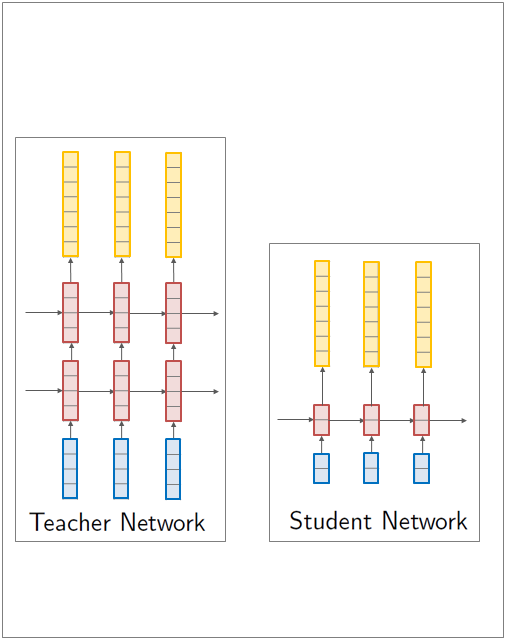
\includegraphics[width=5.5cm]{word-kd-1}
% \end{column}
% \end{columns}
% \end{frame}

% \begin{frame}
%   (Teacher-Student Diagram)
% \end{frame}

\begin{frame}{Application: Model Compression}
  \research{\cite{Kim2016a}}

  \textbf{Goal:} Shrink the size of text generation models.

% \begin{frame}
%   \centerline{\structure{Related Work: Compressing Deep Models}}
% \air

\begin{itemize}
% \item \textbf{Pruning}: Prune weights based on importance criterion
% \cite{LeCun1990,Han2016}
\item Knowledge Distillation: Train a \textit{student} model to learn
from a \textit{teacher} model. %\cite{Bucila2006,Ba2014,Hinton2015}.

\begin{center}
  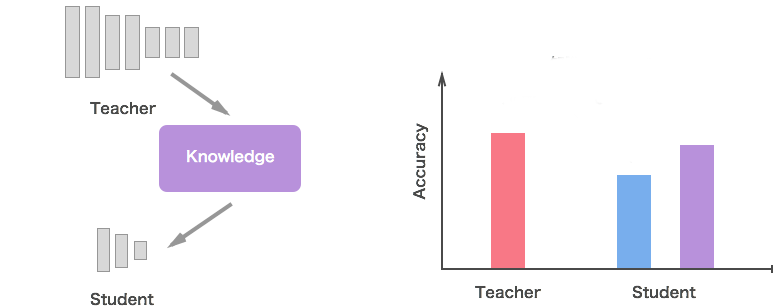
\includegraphics[width=8cm]{distill}
\end{center}
\end{itemize}



% \air
% Other methods:
% \begin{itemize}
% \item low-rank matrix factorization of weight matrices \cite{Denton2014}
% \item weight binarization \cite{Lin2016}
% \item weight sharing \cite{Chen2015}
% \end{itemize}
% \end{frame}



\end{frame}

% \begin{frame}{Baseline}

% \begin{columns}
% \begin{column}{7cm}
% Minimize :
% \air
% $${\cal L}(\theta)-\sum_t \log p(y_t=\hat{y}_t \given \hat{y}_{1:t-1}, x ; \theta)$$

% where $\hat{y}_t$ is the ground truth word at time $t$.

% \air

% Cross-entropy with ground truth.

% \end{column}
% \begin{column}{8cm}
% 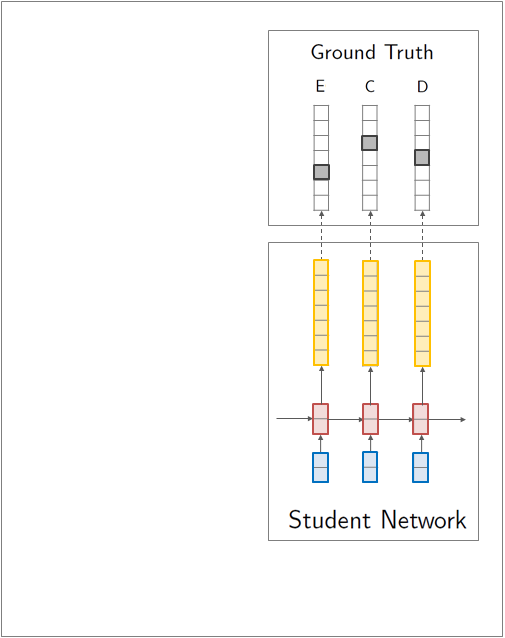
\includegraphics[trim={0.5cm 0.5cm 0.5cm 0.5cm}, clip, width=6cm]{word-kd-0}
% \end{column}
% \end{columns}
% \end{frame}

% \begin{frame}
% \centerline{\structure{Word-Level Knowledge Distillation}}
% \air
% \air
% \begin{columns}
% \begin{column}{6.5cm}
% Teacher network: $q(y_{t} | y_{1:t-1}, \cvec  ; \theta_T$)  \\
% \air
% \air
% Student network: $p(y_{t} | y_{1:t-1}, \cvec; \theta$)
% \end{column}
% \begin{column}{5.5cm}
% 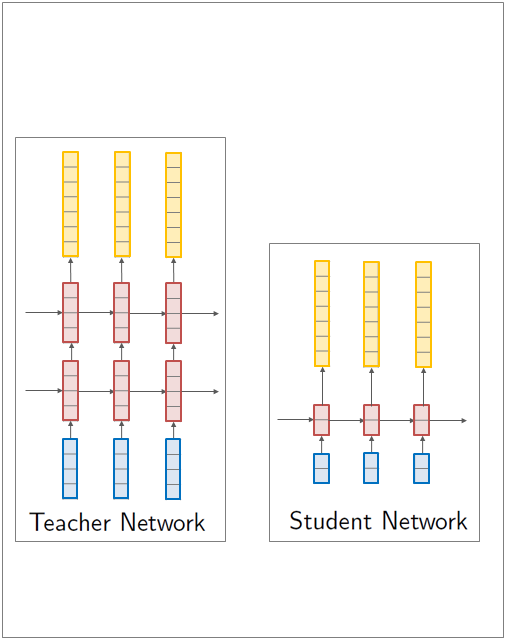
\includegraphics[width=5.5cm]{word-kd-1}
% \end{column}
% \end{columns}
% \end{frame}


\begin{frame}{Multiclass Style: Word-Level Knowledge Distillation}

  \begin{center}
    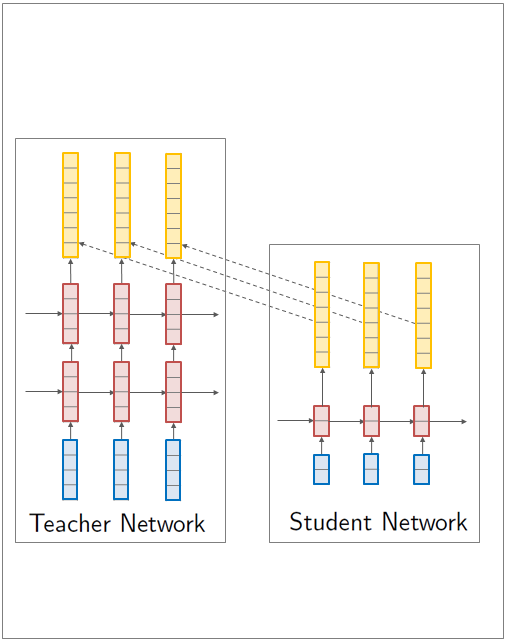
\includegraphics[trim={0.2cm 0.2cm 0.2cm 3cm}, clip,
    width=7cm]{word-kd-2}
  \end{center}
% \begin{columns}
% \begin{column}{7cm}
% Teacher model: $q(y_{t} | y_{1:t-1}, x; \theta_T$)
% \air

% Cross-entropy between teacher and student

% \begin{align*}
% \mathcal{L}_{\text{WORD-KD}}(\theta) = -\sum_t \sum_v &q(y_t=v \given \hat{y}_{1: t-1}, x ; \theta_T)\times \\
% & \log p(y_t =v \given \hat{y}_{1: t-1}, x ; \theta)
% \end{align*}
% \end{column}

% \begin{column}{7cm}
% \centering


% \end{column}
% \end{columns}
\end{frame}

% \begin{frame}
% \centerline{\structure{Word-Level Knowledge Distillation}}
% \air
% \begin{columns}
% \begin{column}{6.5cm}
% Add a term for NLL (equivalent to minimizing cross-entropy between student a mixture distribution of teacher/data distributions)
% \air
% $$\mathcal{L}(\theta) = \alpha\mathcal{L}_{\text{WORD-KD}}(\theta) + (1-\alpha)\mathcal{L}_{\text{NLL}}(\theta)$$
% \air
% $\alpha$ is a hyperparameter (we use $\alpha = 0.5$)
% \end{column}

% \begin{column}{5.5cm}
% 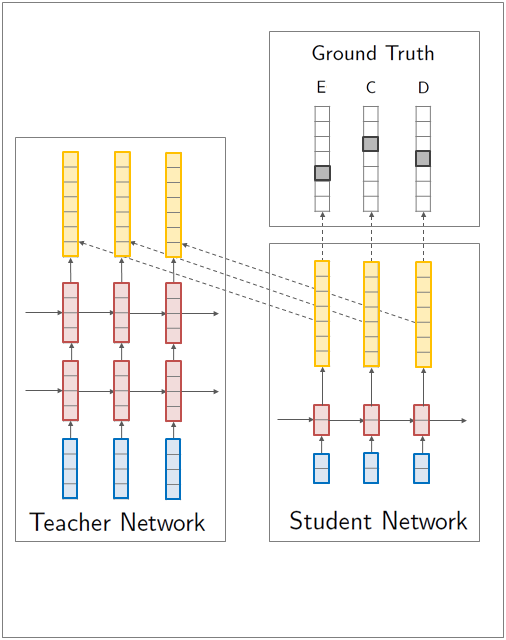
\includegraphics[width=5.5cm]{word-kd-3}
% \end{column}
% \end{columns}
% \end{frame}

% \begin{frame}{Sequence-Level Knowledge Distillation}
% \air
% \air

% \textbf{Motivation:} Replace multiclass with sequence-level cross-entropy.

% \begin{align*}
% \mathcal{L}_{\text{WORD-KD}}(\theta) = -\sum_t \sum_v &q(y_t=v \given \hat{y}_{1: t-1}, x ; \theta_T)\times  \log p(y_t =v \given \hat{y}_{1: t-1}, \cvec ; \theta)
% \end{align*}
% \[ \Downarrow \]
% \[ \mathcal{L}_{\text{SEQ-KD}}(\theta) = -\sum_{v_1} \ldots \sum_{v_T} q(y_{1:T}= v_{1:T}  | x; \theta_T) \times \log p(y_{1:T}=v_{1:T} | x ; \theta)
% \]

% Mimic sequence output of teacher model.
% \air

% Note: bottom distribution is again intractable.


% \end{frame}

% \begin{frame}{Sequence Heuristic Approximation}
% \air
% \air

% %\centerline{Sequence-Level Knowledge Distillation}
% \begin{columns}
% \begin{column}{6cm}
% Approximate $q(y_{1:T} \given x )$ with (beam search) mode sample
% $$q(y_{1:T} \given x ) \approx \mathbf{1}\{\argmax_{y} q(y_{1:T} \given x )\}$$
% % \air
% % $$ y^*_{1:T} \approx  \argmax_{y_{1:T}} q(y_{1:T} \given x ) $$
% % \\
% % Empirically, point estimate captures
% % significant mass

% \end{column}
% \begin{column}{8cm}
% 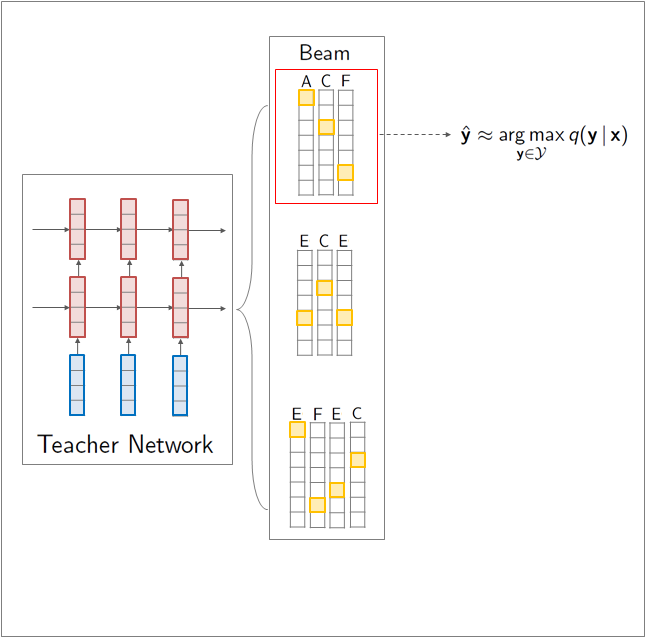
\includegraphics[trim={0.5cm 0.5cm 0.5cm 0.5cm}, clip, width=8cm]{seq-kd-1}
% \end{column}
% \end{columns}
% \end{frame}

\begin{frame}{Sequence-Level Knowledge Distillation}

% \begin{columns}
% \begin{column}{7cm}
% \begin{align*}
% \mathcal{L}_\text{SEQ-KD}(\theta) &= -\log p(y^*_{1:T} \given x ; \theta)  \\
% & \hspace*{-1cm} \displaystyle \approx   -\sum_{v_{1:T}} q(y_{1:T}=v_{1:t}|x; \theta_T) \log p(y_{1:T} | x ; \theta)
% \end{align*}
% \air

% Extension: $\mathcal{L}_\text{SEQ-INTER}(\theta)$ select sample based on ground truth $\hat{y}$
% as well.
% \end{column}
% \begin{column}{7cm}
  \begin{center}
    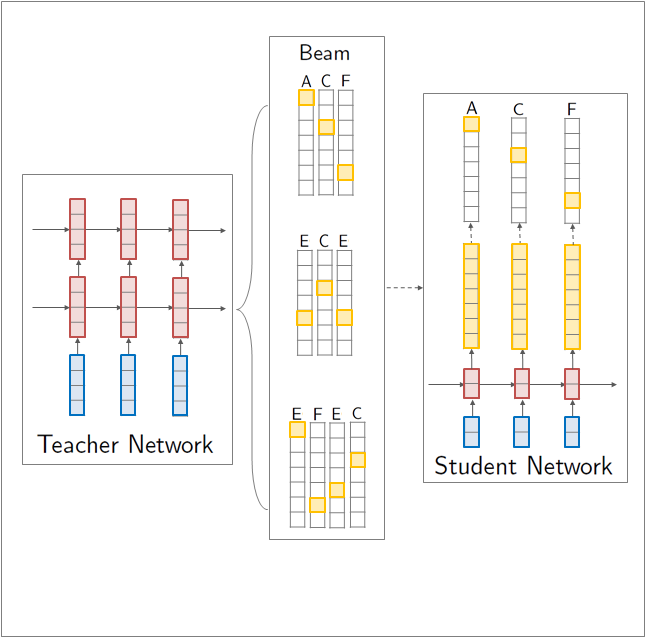
\includegraphics[trim={0.2cm 0.2cm 0.2cm 0.2cm}, clip,
    width=7cm]{seq-kd-2}
  \end{center}
% \end{column}
% \end{columns}
\end{frame}

\begin{frame}{Results: WMT English $\rightarrow$ German Translation}
\air
\air
\begin{table}
\centering
\begin{tabular}{lccccrr}
\toprule
Model &    BLEU$_{K=1}$   & $\Delta_{K=1}$ & BLEU$_{K=5}$ & $\Delta_{K=5}$ \\%& PPL & $p(y^*)$ \\
\midrule
$4 \times 1000$ \\
Teacher    & $17.7$ &  $-$ & $19.5$&   $-$ \\%&   $6.7$ &  $1.3\%$ \\
\midrule
\pause
$2 \times 500$ \\
Student  $\,$   & $14.7$ & $-$ & $17.6$&  $-$ \\%&  $8.2$ & $0.9\%$  \\
\hspace{1mm} Word-KD  & $15.4$ & $+0.7$& $17.7$& $+0.1$\\%&  $8.0$ & $1.0\%$  \\
% \hspace{1mm} Seq-KD   & $18.9$ & $+\mathbf{4.2}$& $19.0$& $+1.4$\\%&  $22.7$ & $                                                                              16.9\%$ \\
\hspace{1mm} Seq-KD  & $18.9$ & $+\mathbf{4.2}$&$19.3$ & $+\mathbf{1.7}$ \\ %&  $15.8$ & $7.6\%$  \\
% \midrule
% \pause
% $4 \times 1000$ \\
% \hspace{1mm} Seq-Inter    & $19.6$ & $+1.9$&  $19.8$& $+0.3$\\ %&   $10.4$ & $8.2\%$   \\
\bottomrule
\end{tabular}

\end{table}
\air
\air
\end{frame}

% \begin{frame}{Combining Knowledge Distillation and Pruning}
% \air
% \air
% \centering
% 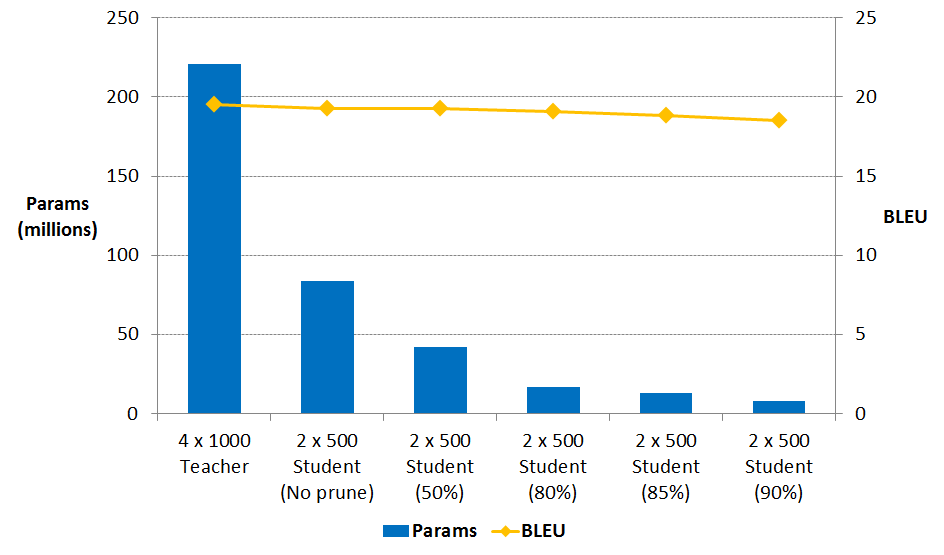
\includegraphics[width=0.8\textwidth]{modelsize}
% \end{frame}


\begin{frame}{Application}

  \begin{center}
    \movie[width=\textwidth, repeat, height=0.85\textheight, width=\textwidth, poster, showcontrols]{Temporary}{videos/translate.mp4}
  \end{center}
\end{frame}

% \begin{frame}{WNMT Translation Scaling Shared Task 2018}
%   (Results)
% \end{frame}
